\documentclass[a4paper,11pt]{article}%
    
\usepackage{fullpage}%
\usepackage[T1]{fontenc}%
\usepackage[utf8]{inputenc}%


\usepackage[french]{babel}% % Adjust the main language


\usepackage{graphicx}%
\usepackage{url}%
\usepackage{abstract}%
\usepackage{lipsum}
\usepackage{mathpazo}%
\usepackage{multicol}
\usepackage{listings}%
\usepackage[linesnumbered,ruled,vlined]{algorithm2e}
\usepackage{subcaption}

\parskip=0.5\baselineskip



\sloppy

\begin{document}

\title{Rapport de stage}

\author{Clément Legrand-Lixon}

\maketitle


\section*{Introduction}
Le Vehicle Routing Problem (VRP), consiste à relier un nombre $n$ de clients par des tournées, commençant et finissant toutes à un même point défini, le dépôt. Ce problème est NP-complet, et dispose de nombreuses applications dans le monde d'aujourd'hui (notamment gestion d'un réseau routier). D'autant plus que ce problème dispose de nombreuses variantes (ajout d'une contrainte de temps, plusieurs dépôts possibles...). L'une des variantes les plus connues consiste à prendre en compte pour chaque client sa demande, de sorte à ce que les tournées créées ne dépassent pas une certaine capacité définie à l'avance. On nomme ce problème Capacitated Vehicle Routing Problem (CVRP). 

Si de nombreuses heuristiques ont vu le jour pour résoudre ce problème, aucune d'entre elles ne parvient à trouver des solutions optimales pour toutes les instances de la littérature, malgré de très bons résultats dans la plupart des cas. Récemment~\cite{Sorensen_2017}, une nouvelle heuristique efficace a vu le jour. L'objectif de mon stage est de s'inspirer de cette heuristique, et d'y intégrer de la connaissance pour rendre l'algorithme plus performant.

Ce rapport commence par présenter le problème étudié, et introduit les notations et opérateurs utilisés dans la suite. Il décrit ensuite comment a été mise en place l'intégration de connaissances au sein de l'algorithme, puis présente les résultats obtenus.   

\section{Présentations}

\subsection{Description du problème}

\subsubsection{Vehicle Routing Problem (VRP)}

Le problème de tournées de véhicules, est un problème NP-complet, qui consiste à déterminer $k$ tournées pour desservir l'ensemble des $n$ clients présents.  Ces tournées doivent toutes passer par un dépôt fixé par l'instance. 
Ainsi les tournées créées doivent respecter les règles suivantes :
\begin{itemize}
\item Chaque client doit être desservi par une et une seule tournée;
\item Chaque tournée doit partir et s'arrêter au dépôt.
\end{itemize}
L'objectif est alors de minimiser la longueur du réseau (ensemble des tournées) et c'est la distance euclidienne, qui est privilégiée pour la majorité des instances. 
Un exemple d'instance est présenté en figure~\ref{Instance3205}, où les points rouges représentent les clients et le point bleu le dépôt. Une solution possible au problème est représenté en figure~\ref{SNC3205} mais n'est à priori pas optimale. 
De nombreux algorithmes ont vu le jour pour tenter de résoudre ce problème, ainsi que les nombreuses variantes qui existent (ajout de contraintes de capacité, temps ou longueur sur les tournées, ces contraintes sont cumulables). 
C'est l'ajout de capacité aux tournées qui nous intéressera plus particulièrement.


\begin{figure}

\centering
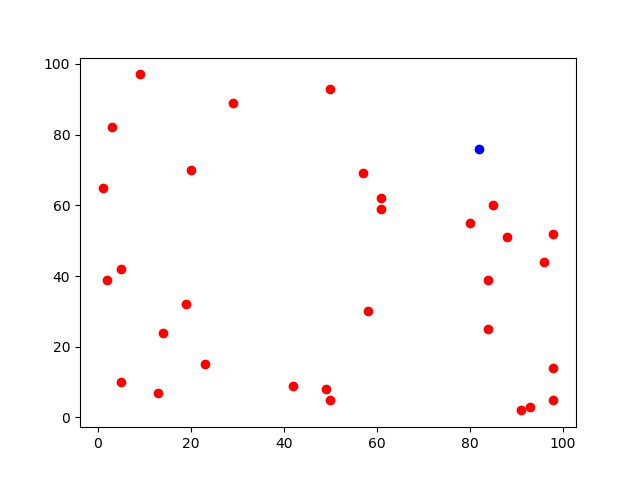
\includegraphics[scale=0.5]{Instance.png}
\caption{Représentation de l'instance A-n32-k05 de la littérature}
\label{Instance3205}
\end{figure}

\begin{figure}

\centering
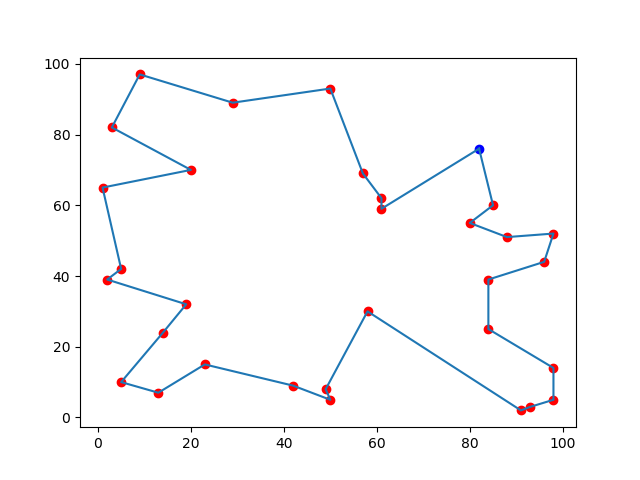
\includegraphics[scale=0.5]{solutionNoCapacity.png}
\caption{Représentation d'une solution de l'instance A-n32-k05}
\label{SNC3205}
\end{figure}

\subsubsection{Capacitated VRP (CVRP)}

L'une des extensions les plus étudiées du VRP, est celle où l'on rajoute une contrainte de capacités sur les tournées, cette contrainte étant la même pour toutes les tournées. 
Dorénavant, chaque client a une certaine demande, mais la demande présente sur une tournée ne doit pas excéder la capacité disponible sur celle-ci.
Les tournées doivent donc respecter la règle suivante, en plus de celles décrites à la section précédente :
\begin{itemize}
\item La demande totale sur chaque tournée ne doit pas excéder la capacité disponible.
\end{itemize}
Si on reprend l'instance A-n32-k05, en considérant les demandes des clients ainsi que la capacité disponible pour chaque véhicule, on obtient une solution présente sur la figure~\ref{SC3205}, qui n'est pas optimale. 
Ce problème est beaucoup étudié car il a de nombreuses applications (comme par exemple la gestion du trafic routier, ou alors la gestion d'un réseau de bus), et peu de solutions optimales ont été trouvées pour des instances de plus de $500$ clients. 

\begin{figure}
\centering
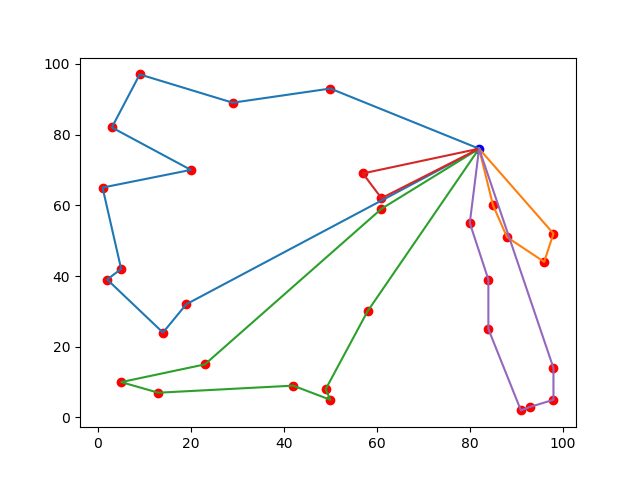
\includegraphics[scale=0.5]{solutionCapacity.png}
\caption{Représentation d'une solution de l'instance A-n32-k05, où les demandes des clients sont prises en compte}
\label{SC3205}
\end{figure}

\subsection{Parcours et exploration des voisinages}
\label{voisinage}

Lorsqu'il s'agit de trouver une solution optimale à un problème, il est souvent intéressant d'explorer les voisinages d'une solution pour voir s'il n'y a pas mieux. Selon la méthode d'exploration employée, il peut être intéressant de parcourir le voisinage de différentes manières, pour ne pas toujours favoriser les mêmes voisins.

L'\underline{exploration} d'un voisinage de solutions peut être plus ou moins exhaustif selon la condition d'arrêt utilisée.
On distingue principalement, deux conditions d'arrêt lorsqu'il s'agit d'explorer des voisinages :

\begin{itemize}
\item First improvement (\emph{FI}) : on parcourt le voisinage jusqu'à trouver un changement qui améliore la solution actuelle (on s'arrête donc à la première amélioration trouvée);
\item Best improvement (\emph{BI}) : on parcourt tout le voisinage, et on applique le changement qui va le plus améliorer notre solution actuelle. \\
\end{itemize}

Pour explorer un voisinage, on peut le \underline{parcourir} de différentes manières de sorte à ne pas toujours favoriser les mêmes voisins. On considérera ici 3 parcours différents : 

\begin{itemize}
\item Dans l'ordre (\emph{O}) : les voisins sont parcourus dans un ordre naturel (du premier au dernier);
\item Dans un semi-ordre (\emph{SO}) : on commence le parcours là où on s'était arrêté au dernier parcours, on parcourt ensuite les voisins dans l'ordre;
\item Aléatoirement (\emph{RD}) : on tire aléatoirement l'ordre dans lequel on va parcourir les voisins. \\
\end{itemize}

On peut remarquer que peu importe le parcours effectué, pour faire une exploration \emph{BI}, il faudra passer par tous les voisins. Pour qu'une exploration \emph{FI} soit efficace, il faut éviter un parcours \emph{O}, car dans ce cas on privilégie une certains voisinages qui seront choisis plus souvent. On retiendra le tableau récapitulatif suivant:

\begin{center}
\begin{tabular}{|c|c|c|}
   \hline
     & \emph{BI} & \emph{FI}  \\
   \hline
   \emph{O} & Oui & Non \\
   \hline
   \emph{SO} & Non & Oui \\
   \hline
   \emph{RD} & Non & Oui  \\
   \hline
\end{tabular}
\end{center}


\subsection{Les constituants de l'algorithme}
Cette partie décrit l'ensemble des briques utilisées pour construire l'algorithme. Ces briques dépendent du problème étudiée (ici CVRP), mais sont indépendantes entre elles. De fait, il est possible de construire de nombreux algorithmes en les empilant de différents manières.

\subsubsection{Condition d'arrêt}

Lors de la recherche d'une solution optimale d'un problème, il est indispensable de s'intéresser à la condition d'arrêt de l'heuristique utilisée. En effet, on doit trouver un compromis entre temps de calcul et qualité de la solution recherchée. On ne peut jamais être totalement sûr que la solution obtenue est bien optimale, mais on ne peut pas non plus explorer l'intégralité des solutions. Les principales conditions d'arrêt rencontrées sont les suivantes :
\begin{itemize}
\item Un certain temps d'itérations sans solutions améliorantes à ne pas dépasser (3 minutes dans l'article~\cite{Sorensen_2017});
\item Un nombre d'itérations sans solutions améliorantes à ne pas dépasser (de l'ordre de $n^2$ dans mon algorithme). 
\end{itemize}

\subsubsection{Initialisation}
Avant de pouvoir appliquer l'heuristique, il faut pouvoir déterminer une solution initiale sur laquelle les modifications vont être appliquées. 

Cette solution peut être créée de différentes manières:

\begin{itemize}
\item Elle peut être générée aléatoirement (Alea);
\item Elle peut être obtenue grâce à l'algorithme de Clarke \& Wright (CW) (algorithme \ref{algo:CW}), avec les paramètres ($\lambda,\mu,\nu$)~\cite{Altinel_2005}. Les savings se calculent via la formule suivante:

\begin{center}
$s(i,j) = c_{i0} + c_{0j} - \lambda c_{ij} + \mu \vert c_{i0} - c_{0j} \vert + \nu \frac{d_i + d_j}{\overline{d}}$
\end{center}

où $c_{ij}$ dénote la distance entre les clients $i$ et $j$ (le client 0 étant le dépôt), et $d_i$ dénote la demande du client $i$. 

L'intérêt de cet algorithme est qu'il donne une bonne solution initiale en peu de temps, ce qui permet de l'exécuter un grand nombre de fois rapidement.
\item Elle peut être calculée grâce à l'intégration de connaissances (Learn). C'est ce dernier point que nous tenterons de mettre en œuvre par la suite.
\end{itemize}

\begin{algorithm}
\DontPrintSemicolon % Some LaTeX compilers require you to use \dontprintsemicolon instead
\KwIn{Un ensemble de points I, un ensemble d'entiers $D = {d_1,...,d_n}$ et un triplet $(\lambda,\mu,\nu)$ de flottants}
\KwOut{Une solution au problème I}

\For{$i \gets 1$ \textbf{to} $n$} {
	$Sol \gets Sol \cup [0,i,0]$\;
}
Calculer les savings de toutes les arêtes\;

\While{le saving maximal est positif} {
	$(i,j) \gets argmax_{(i,j)} s(i,j)$\;
	$r_i \gets findRoute(Sol,i)$\;
	$r_j \gets findRoute(Sol,j)$\;
	\If{$r_i$ et $r_j$ peuvent fusionner} {
		Retirer $r_i$ et $r_j$ de $Sol$\;
		Fusionner $r_i$ et $r_j$\;
		Ajouter le résultat dans $Sol$ et mettre $s(i,j) = 0$\;
	}
}

\Return{$Sol$}\;
\caption{{\sc Clarke-Wright} calcule une solution initiale}
\label{algo:CW}
\end{algorithm}

\subsubsection{Pire arête et pénalisation}
A chaque tour de boucle, on calcule l'arête $(i,j)$ qui maximise la fonction suivante (donnée dans l'article):
\begin{center}
$b(i,j) = \frac{[\lambda_w w(i,j) + \lambda_c c(i,j)] [\frac{d(i,j)}{max_{k,l}d(k,l)}] ^ {\frac{\lambda_d}{2}}}{1+p(i,j)}$
\end{center}
où:
\begin{itemize}
\item $p(i,j)$ est la pénalisation de l'arête $(i,j)$ (nombre de fois où l'arête a maximisé $b$);
\item $w(i,j)$ est la largeur de l'arête $(i,j)$;
\item $c(i,j)$ est le coût de l'arête $(i,j)$ ($c(i,j) = c_{ij}(1 + \lambda p(i,j)$, avec $\lambda = 0.1$ dans l'article);
\item $d(i,j)$ est la profondeur de l'arête $(i,j)$ (max de $c_{0i}$ et $c_{0j}$);
\item les paramètres $\lambda_w,\lambda_c,\lambda_d$, prennent comme valeurs $0$ ou $1$, selon les caractéristiques que l'on veut considérer. Il y a ainsi 6 fonctions de pénalisation différentes, que l'on peut choisir au cours de l'exécution (on ne considère pas le cas où $\lambda_w = \lambda_c = 0$, puisqu'il fournit $b(i,j) = 0$.

\end{itemize}

C'est autour de l'arête calculée ici que vont s'orienter les recherches des opérateurs locaux qui suivent.
 
\subsubsection{Ejection-Chain}

Cet opérateur va essayer de déplacer au plus $l$ clients sur des tournées plus adaptées. Dans l'article~\cite{Sorensen_2017} $l = 3$. En effet l'algorithme~\ref{algo:EC}, qui décrit le fonctionnement de cet opérateur, s'exécute en $O(n^{l-1})$. Il vaut donc mieux choisir une valeur de $l$ assez petite, pour que la complexité n'explose pas. 

\begin{algorithm}
\DontPrintSemicolon % Some LaTeX compilers require you to use \dontprintsemicolon instead
\KwIn{Une arête $(a,b)$, la liste des plus proches voisins des clients $voisins$, un entier $l$, la solution actuelle $sol$}
\KwOut{Une nouvelle solution au moins aussi bonne que $sol$}
$possibleSol \gets sol$\;
$cand \gets choose(a,b)$\;
$nextRoute \gets findNextRoute(cand,voisins,possibleSol)$\;
$possibleSol \gets $ déplacer $cand$ après son voisin sur $nextRoute$\;
\For{$i \gets 1$ \textbf{to} $l-1$} {
  $cand \gets $un client de $nextRoute$ différent de celui ajouté\;
  $nextRoute \gets findNextRoute(cand,voisins,possibleSol)$\;
  $possibleSol \gets$ déplacer $cand$ après son voisin sur $nextRoute$\;
}
\If {$cost(possibleSol) < cost(sol)$} {
	$sol \gets possibleSol$\;
}
\Return{$sol$}\;
\caption{{\sc Ejection-Chain} applique l'opérateur ejection-chain}
\label{algo:EC}
\end{algorithm}

Aux lignes $3, 4, 7$ et $8$ de l'algorithme~\ref{algo:EC}, il est possible d'utiliser les méthodes de la section~\ref{voisinage} pour explorer les voisinages.

\subsubsection{Cross-Exchange}

Cet opérateur essaie d'échanger deux séquences de clients successifs entre deux tournées. Il est possible de limiter le nombre de clients par séquence échangée.
L'algorithme~\ref{algo:CE} présente l'exécution de l'opérateur et s'exécute en $O(n^2)$.

\begin{algorithm}
\DontPrintSemicolon % Some LaTeX compilers require you to use \dontprintsemicolon instead
\KwIn{Une arête $(c_1,c_2)$, la liste des plus proches voisins des clients $voisins$, la solution actuelle $sol$}
\KwOut{Une nouvelle solution au moins aussi bonne que $sol$}
$possibleSol \gets sol$\;
$nextRoute \gets findNextRoute(c_1,voisins,possibleSol)$\;
Considérer l'arête $(c_3,c_4)$ de $nextRoute$, où $c_4$ est le proche voisin de $c_1$ utilisé\;
$possibleSol \gets exchange(c_1,c_3,possibleSol)$\;
Choisir 2 clients $c_5$ et $c_6$ qui n'appartiennent pas à la même tournée\;
$possibleSol \gets exchange(c_5,c_6,possibleSol)$\;
\If {$cost(possibleSol) < cost(sol)$} {
	$sol \gets possibleSol$\;
}
\Return{$sol$}\;
\caption{{\sc Cross-Exchange} applique l'opérateur cross-exchange}
\label{algo:CE}
\end{algorithm}

A la ligne $6$ de l'algorithme~\ref{algo:CE}, il est possible d'utiliser les méthodes de la section \ref{voisinage} pour explorer les voisinages, et choisir les clients à échanger.

\subsubsection{Lin-Kernighan}

L'heuristique Lin-Kernighan est utilisé en général pour résoudre le problème du voyageur de commerce (TSP). Il effectue une optimisation intra-tournée (c'est-à-dire que la tournée considérée est améliorée indépendamment des autres). 
Cela consiste en une réorganisation des clients sur la tournée. On choisit $k$ tel que \emph{LK} ne dépasse pas \emph{k-opt} au cours de son exécution. 
On appelle \emph{k-opt}, l'opération qui consiste à échanger $k$ clients différents sur la tournée. 
On commence alors par appliquer 2-opt, si une amélioration est trouvée, on passe à 3-opt, et ainsi de suite jusqu'à atteindre k-opt. 
On repart alors de 2-opt, et ce jusqu'à ne plus trouver d'améliorations. 
D'après l'article~\cite{Sorensen_2017}, on peut prendre $k = 2$.
L'algorithme~\ref{algo:LK} décrit l'exécution de l'opérateur.

\begin{algorithm}
\DontPrintSemicolon % Some LaTeX compilers require you to use \dontprintsemicolon instead
\KwIn{Une tournée $r$ à améliorer}
\KwOut{Une permutation de $r$ ayant un meilleur coût que $r$}
$r_{next} \gets 2$-$opt(r) $\;
\While{$ r_{next} \neq r$} {
  $r \gets r_{next}$\;
  $r_{next} \gets 2$-$opt(r)$\;
}
\Return{$r$}\;
\caption{{\sc Lin-Kernighan} applique l'opérateur Lin-Kernighan}
\label{algo:LK}
\end{algorithm}

Lorsqu'il s'agit d'appliquer \emph{2-opt}, il est possible d'utiliser les méthodes de la section \ref{voisinage} pour explorer les voisinages.

\subsection{Algorithmes mis en œuvre}
Les algorithmes présentés précédemment peuvent être enchaînés dans l'ordre que l'on veut. 
En effet, seule le résultat obtenu importe, les algorithmes sont donc indépendants. 
Nous présentons ici l'algorithme utilisé par Arnold et S\"\o rensen dans~\cite{Sorensen_2017}, ainsi que l'algorithme que nous utiliserons pour la suite.

\subsubsection{Heuristique d'Arnold et Sörensen}

L'heuristique décrite par Arnold et Sörensen est présentée dans l'algorithme~\ref{algo:AS}. 
Elle est à la fois déterministe et efficace, c'est-à-dire qu'elle trouve de bonnes solutions pour de nombreuses instances en un temps raisonnable. 
Les auteurs pré-calculent également les $30$ plus proches voisins de chacun des clients.


\begin{algorithm}
\DontPrintSemicolon % Some LaTeX compilers require you to use \dontprintsemicolon instead
\KwIn{Un ensemble de points I, les demandes des clients D, un triplet de flottants $(\lambda,\mu,\nu)$}
\KwOut{Une solution au problème I}
$Sol \gets CW(I,D,\lambda,\mu,\nu)$\;
$N \gets length(D)$\;
$nextSol \gets Sol$\;
\While {Pas 3 minutes depuis la dernière amélioration} {
	$worstEdge \gets argmax_{(i,j)} b(i,j) $\;
	$nextSol \gets EC_{BI-O}(worstEdge,I,D)$\;
	Améliorer chaque tournée avec $LK_{BI-O}$\;
	$nextSol \gets CE_{BI-O}(worstEdge,I,D)$\;
	Améliorer chaque tournée avec $LK_{BI-O}$\;
	\If {$cost(Sol) > cost (nextSol)$} {
		$ Sol \gets nextSol$\;
	}
	\If {Pas d'améliorations depuis $N/10$ itérations} {
		Appliquer les opérateurs sur toutes les arêtes de la solution\;
	}
	\If {Pas d'améliorations depuis $20N$ itérations} {
		Changer de fonction de pénalisation en prenant un autre triplet $(\lambda_w,\lambda_c,\lambda_d)$\;
	}
	\If {Pas d'améliorations depuis $100N$ itérations} {
		Réinitialiser les pénalités des arêtes\;
	}
}
\Return{$Sol$}\;
\caption{{\sc AS} applique l'heuristique A\& S au problème considéré}
\label{algo:AS}
\end{algorithm}



\subsubsection{Algorithme utilisé}

Il est possible de construire de nombreuses variantes de l'algorithme précédent, selon l'ordre dans lequel on exécute les opérateurs. 
Après avoir testé quelques possibilités, c'est finalement l'algorithme~\ref{algo:A} que nous retiendrons. 
Il permet en effet le parcours de nombreux voisinages, puisqu'ils sont choisis aléatoirement. 
Mais le temps d'exécution est plus long, car les solutions obtenues étant aléatoires, nous exécutons $20$ fois l'algorithme. 
Cela permet d'obtenir le coût moyen d'une solution renvoyée, et nous retenons la meilleure solution trouvée lors des $20$ exécutions. 


\begin{algorithm}
\DontPrintSemicolon % Some LaTeX compilers require you to use \dontprintsemicolon instead
\KwIn{Un ensemble de points I, les demandes des clients D, un triplet de flottants $(\lambda,\mu,\nu)$}
\KwOut{Une solution au problème I}
$Sol \gets CW(I,D,\lambda,\mu,\nu)$\;
Améliorer chaque tournée avec $LK_{BI-O}$\;
$N \gets length(D)$\;
$nextSol \gets Sol$\;
\While {Pas 1 minute depuis la dernière amélioration} {
	$worstEdge \gets argmax_{(i,j)} b(i,j) $\;
	$nextSol \gets EC_{FI-RD}(worstEdge,I,D)$\;
	Améliorer chaque tournée avec $LK_{BI-O}$\;
	$nextSol \gets CE_{FI-RD}(worstEdge,I,D)$\;
	Améliorer chaque tournée avec $LK_{BI-O}$\;
	\If {$cost(Sol) > cost (nextSol)$} {
		$ Sol \gets nextSol$\;
	}
	\If {Pas d'améliorations depuis $N/2$ itérations} {
		$nextSol \gets Sol$\;
	}
	\If {Pas d'améliorations depuis $2N$ itérations} {
		Changer de fonction de pénalisation en prenant un autre triplet $(\lambda_w,\lambda_c,\lambda_d)$\;
		Réinitialiser les pénalités des arêtes\;
		Améliorer chaque tournée de $Sol$ avec $LK_{BI-O}$\;
	}
}
\Return{$Sol$}\;
\caption{{\sc A} calcule une solution du problème considéré}
\label{algo:A}
\end{algorithm}


\section{Utilisation de connaissances}

Maintenant que nous disposons d'un algorithme performant pour calculer des solutions aux instances considérées, nous allons essayer d'extraire de la connaissance à partir des solutions initiales fournies par Clarke-Wright, pour les intégrer ensuite à l'algorithme A.
 
\subsection{Motivation}


\subsection{Extraction des connaissances}
décrire algo d'apprentissage + résultats

\subsection{Intégration des connaissances}
décrire nouvel algo + résultats


\bibliographystyle{plain}
\bibliography{biblio}

\end{document}